\documentclass[12pt,a4paper,titlepage]{article}
% enlever twoside pour la version pdf
\usepackage[a4paper,hmarginratio=2:2]{geometry}
\usepackage[french]{babel}
\usepackage[utf8]{inputenc}
\usepackage[T1]{fontenc}
\usepackage{lmodern}
\usepackage{epsfig}
\usepackage{wrapfig}
\usepackage{thmbox} % theorem box (joli theoreme)
% \usepackage{amsthm} % theorem
\usepackage{setspace} % theorem interline
\usepackage{amssymb}
\usepackage{amsmath}
\usepackage{alltt}
\usepackage[backref=page,plainpages = false]{hyperref}
\usepackage{parskip}
\usepackage{verbatim}
\usepackage{listings}
%\usepackage{marvosym}
\usepackage{fancyhdr}
\usepackage{color}

\pagestyle{fancy}
\fancyhead[LE,RO]{\thepage}
\fancyfoot{}

% define custom color
\definecolor{red75}{rgb}{0.75,0,0}
\definecolor{blue50}{rgb}{0,0,0.5}

% theorem list
% \newtheorem{mydef}{Definition}

\renewcommand{\labelitemi}{\textbullet}
\setlength{\parindent}{0cm} % pas d'alinéa





\title{Rapport du projet d'AAW :\\ 
Réseau social en Java J2EE.}
\author{William Le Coroller \& Romain Boutin}
\date{Mercredi 25 Février 2015}

\begin{document}
\pagenumbering{Roman}



% - - - - - - - début de la page de garde - - - - - - - - - - - - - - - - - - -



\thispagestyle{empty}

\maketitle

\clearpage{\pagestyle{empty}}



% - - - - - - - fin de la page de garde - - - - - - - - - - - - - - - - - - - -



\clearpage{\pagestyle{empty}}

\tableofcontents
\clearpage{\pagestyle{empty}}

\pagenumbering{arabic}



% ========== nouvelle page ====================================================



\clearpage{\pagestyle{empty}}



\section{Introduction}

Le but de ce projet est la réalisation d'un réseau social en utilisant les technologies
Java J2EE.\\

Le rapport est organisé en trois parties principales :
\begin{itemize}
\item La partie \begin{bf}contexte\end{bf} qui présente les points que le projet doit respecter.

\item La partie \begin{bf}technique\end{bf} qui présente les choix techniques qui ont été effectués.

\item La partie \begin{bf}conception\end{bf} qui présente la conception des différentes couches
de l'application.
\end{itemize}



% ========== nouvelle page ====================================================



\clearpage{\pagestyle{empty}}



\section{Contexte}
Le but de ce projet est de concevoir et implanter un réseau social simplifié.\\
Les contraintes suivantes nous ont été imposées :
\begin{itemize}
\item Chaque utilisateur est enregistré en base de données.
\item Chaque utilisateur dispose d'une liste d'amis qui lui est associé.
\item Chaque utilisateur pourra partager des fichiers avec ses amis.
\item Chaque liste d'amis des utilisateurs est enregistré en base de données.
\item Chaque utilisateur a la possibilité d'échanger des messages avec ses amis.
\item Chaque utilisateur a la possibilité d'identifier ses amis dans ses publications.
\item Dès lors il sera notifié d'une telle identification.
\end{itemize}



% ========== nouvelle page ====================================================



\clearpage{\pagestyle{empty}}



\section{Choix techniques}
Nous avons choisi d'utiliser comme technologies la combinaison des Enterprise JavaBeans (EJB)
et JavaServer Faces (JSF). En effet, ces technologies nous ont parut plus intuitive et solide 
que leurs homologues JPA et Spring. L'utilisation redondante de JavaBeans étant indéniablement 
un atout en terme d'évolutivité et de maintenabilité.



% ========== nouvelle page ====================================================



\clearpage{\pagestyle{empty}}



\section{Conception}

\subsection{Modèle base de données}

\textbf{Table T\_USER}\\
Cette table décrit l'ensemble des informations des utilisateurs inscrit sur le 
réseau social.\\
\newline

\textbf{Table T\_RELATIONSHIP}\\
Cette table décrit l'ensemble des informations permettant d'établir une relation 
d'amitié entre deux utilisateurs inscrit sur le réseau social.\\
\newline

\textbf{Table T\_NOTIFICATION}\\
Cette table recense l'ensemble des notifications des différents utilisateurs du réseau 
social.\\
\newline

\textbf{Table T\_MESSAGE}\\
Cette table regroupe l'ensemble des messages publiques et privés échangés par les 
utilisateurs du réseau social.\\



% ========== nouvelle page ====================================================



\clearpage{\pagestyle{empty}}



\subsection{Diagramme de classe}

\begin{figure}[ht]
	\centering
	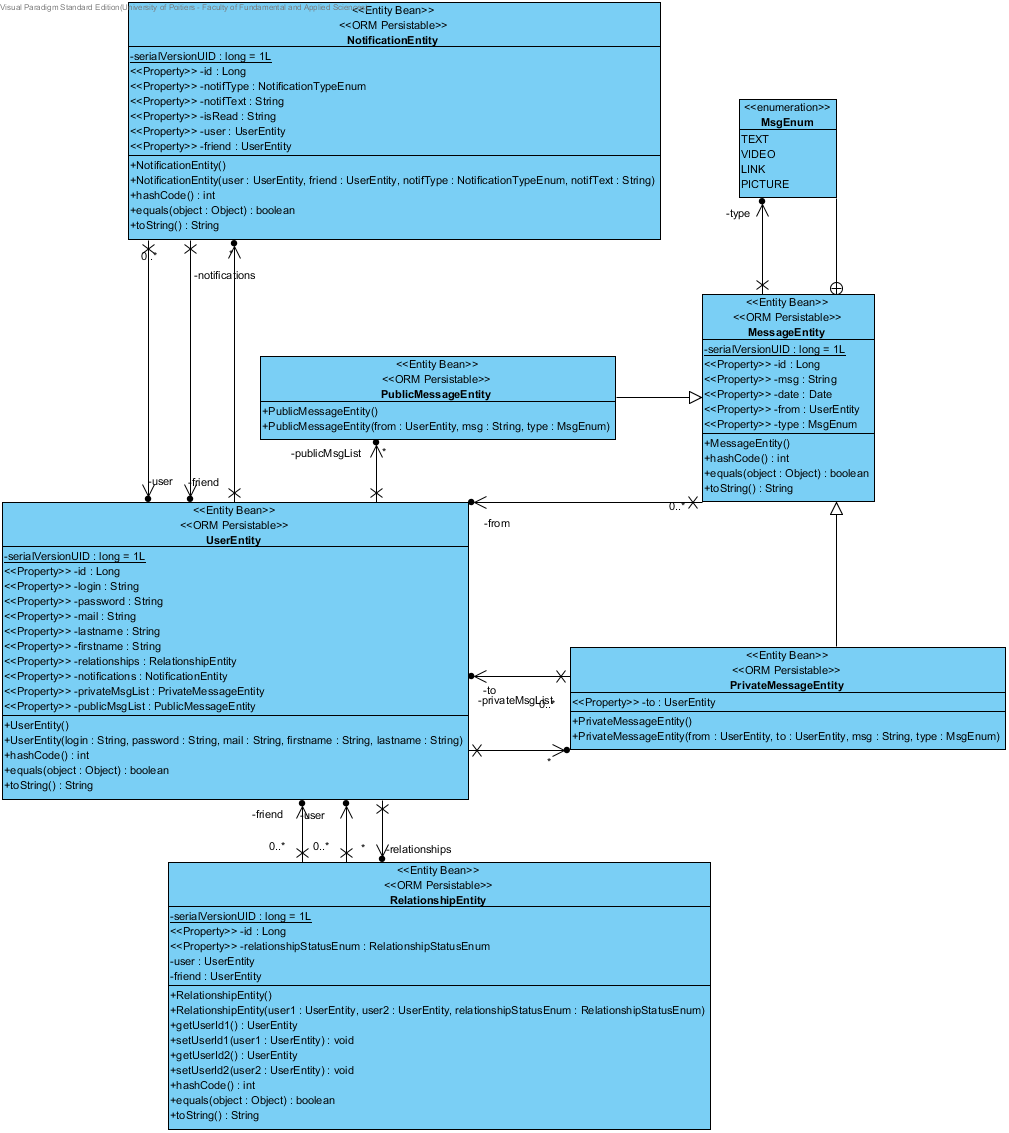
\includegraphics[width=13cm]{img/Class_Diagram_Entity.png}
	\caption{Le diagramme de classe associé au package \og{}entity\fg{}}
\end{figure}



% ========== nouvelle page ====================================================



\clearpage{\pagestyle{empty}}



\subsection{Couche DAO}
La couche DAO effectue l'interfaçage entre la base de données et la couche service/métier.
Elle fourni au travers des entités et des Entreprise JavaBeans une modélisation des données 
stockées dans la base de données.

\textbf{Package Entity}\\
Les classes présentes dans ce package sont les classes \og{}entités\fg{}. Ces classes 
donnent un cadre uniforme pour l'accès aux données en réalisant un mapping des différentes
tables présentent en base de données.\\

\begin{itemize}
\item \textbf{MessageEntity}, \textbf{PublicMessageEntity} et \textbf{PrivateMessageEntity} : Ces classes représentent la table \og{}T\_MESSAGE\fg{}.
\item \textbf{NotificationEntity} : Cette classe représente la table \og{}T\_NOTIFICATION\fg{}.
\item \textbf{RelationshipEntity} : Cette classe représente la table \og{}T\_RELATIONSHIP\fg{}.
\item \textbf{UserEntity} : Cette classe représente la table \og{}T\_USER\fg{}.\\
\end{itemize}

\textbf{Package SessionBeanLocal et SessionBean}\\
Les classes présentes dans ce package sont les interface local des Beans de session 
propre à EJB.\\
\newline
L'ensemble des classes de ce package présente une interface assez similaire avec 
la déclaration des méthodes \og{}save\fg{}, \og{}update\fg{} et \og{}delete\fg{} 
permettant respectivement de sauvegarder ou créer, de mettre à jour ou de détruire 
une entité et de répercuter ce changement en base de données à l'aide d'un objet 
\og{}EntityManger\fg{}.\\
\newline



% ========== nouvelle page ====================================================



\clearpage{\pagestyle{empty}}



\subsection{Couche Service}
Aussi appelé \og{}couche métier\fg{}, elle fait le lien entre la couche présentation et la couche DAO.
Avec EJB, cette couche se résume à l'implémentation de JavaBeans dit de service fournissant donc des 
méthodes de plus haut niveau afin de traité les requêtes utilisateurs plus simplement.
\newline

\textbf{Package BeanLocal et Bean}\\
L'implémentation a été effectué de telle sorte que pour chaque fonctionnalité est associé 
le service correspondant. On voit bien ici la force des EJB.
\newline

\subsection{Couche Présentation}
Il s'agit de la couche la plus proche de l'utilisateur. C'est elle qui présente à l'utilisateur 
l'ensemble des actions, via des pages web, qu'il peut effectuer.
\newline

\textbf{Package ManagedBeans}\\
Pour un soucis de gestion de session il a été décidé de créer un managedBean plus important.
Les autres managedBeans représentent des fonctionnalités indépendantes de l'utilisateurs.
\newline

\textbf{Gestion des messages}\\
On a choisi par simplicité d'imposer à l'utilisateur de poster des vidéos ou des photos 
via des liens de fichiers déjà uploadé. On applique juste un traitement sur les différents 
liens pour les afficher correctement.



% ========== nouvelle page ====================================================



\clearpage{\pagestyle{empty}}



\section{Conclusion}
La quasi-totalité des fonctionnalitées attendues ont été implémentées à l'exception 
de l'identification d'un amis dans un message.\\
Le réseau social est fonctionnel bien qu'austère. Il respecte l'ensemble des directives 
d'implémentation des technologies J2EE traitées en cours.\\
On regrette néanmoins de ne pas avoir pu rajouté des fonctionnalités de confort ainsi 
que de vérification afin de rendre l'expérience utilisateur plus ergonomique et intuitive.\\




% ========== nouvelle page ====================================================



\clearpage{\pagestyle{empty}}



\end{document}